\documentclass[conference]{IEEEtran}

\usepackage{cite}
\usepackage{float}
\usepackage{hyperref}
\usepackage{graphicx}
\graphicspath{ {./Assets/} }


\title{Automatic User Profiling for Intelligent Tourist Trip Personalisation}

\author{\IEEEauthorblockN{Liam Attard [0299300L] }
\IEEEauthorblockA{Department of Artificial Intelligence}
\textit{University of Malta}\\
\textit{liam.attard.18@um.edu.mt}}

\begin{document}

  \maketitle

  \begin{abstract}
    lorem ipsum dolor sit amet, consectetur adipiscing elit, sed do
    eiusmod tempor incididunt ut labore et dolore magna aliqua. Ut
    enim ad minim veniam, quis nostrud exercitation ullamco laboris
    nisi ut aliquip ex ea commodo consequat. Duis aute irure dolor in
    reprehenderit in voluptate velit esse cillum dolore eu fugiat
    nulla pariatur. Excepteur sint occaecat cupidatat non proident,
    sunt in culpa qui officia deserunt mollit anim id est laborum.
  \end{abstract}

  \begin{IEEEkeywords}
  tourism,itinerary, user-profiling.
  \end{IEEEkeywords}

  \section{Introduction}
    \subsection{Problem Definition}

        Producing an itinerary before a trip can be a demanding task
        which requires  a substantial amount of  research. Many times
        people rely on travel books, individual travel blogs and online
        websites to form a holiday plan, but these are not always tailored according 
        to the traveller’s preferences and opinions \cite{DeChoudhury2010}. 

        An adequate automated trip planner application would consist
        of two parts, 
        
        \begin{enumerate}
                \item the retrieval of user preferences 
                \item the generation of a custom itinerary
        \end{enumerate}
        Numerous systems are available and 
        therefore building a working prototype is both possible and feasible 
        \cite{Sylejmani2017,Chang2016,Sylejmani2012,Sebastia2009a,Tumas2009,
        Vansteenwegen2011,Kurata2013, RamalhoBrilhante2014, 
        DeChoudhury2010,DUNSTALL2008a, DiBitonto2010a,Gavalas }. 
        Although these systems automate the process of producing the 
        itinerary, they require a lot of end-user data and preferences 
        to form a personalised itinerary. Can the user preference 
        gathering be automated?

        Given the amount of information a single user holds online, 
        it is possible to automate and help the process of 
        gathering personal preferences \cite{Buraya2017}. A deep 
        learning model could be trained to classify a person's social
        media profile to determine what the user wants from a trip. 
        This information alongside other parameters such as the user's
        budget and trip length could give out a very accurate 
        personalised holiday plan.

\subsection{Motivation}
        The immense amount of data generated by each user online \cite{J.Clement2020} 
        alongside the benefits that a tourist recommender system brings 
        were the two main motivators behind this project. If a user allows 
        the system to gather preferences based on his social media profile
        and provides a small number of additional preferences such as
        the budget and destination, a personalised itinerary could be
        generated automatically.
\subsection{Why the Problem is non-trivial}

  \section{Background Research and Literature Review}
    Several studies both on user profiling and on real-time automatic trip
itinerary generation have been carried out throughout the years. 

There are many types of systems which help the travellers in their
trips. Gavalas et al. \cite{Gavalas2014} categorised these into
\textbf{POI recommenders, Tourist Service Recommenders, Collaborative
content from users and social media services, path recommenders} and
\textbf{Personlised multiple-day tour planners}. The planning of a
trip to a traveller introduces the Tourist Trip Design Problem (TTDP)
which has recieved a lot of observation and heuristic contribution
\cite{Gunawan2016,Delic2018}. Sylejmani et al.\cite{Sylejmani2017} have defined
the TTDP as part of the Orienteering Problem(OP). OP problems contain
a number of nodes each containing a score and try to solve the path
containing the maximal score constrained with parameters such as time
and budget \cite{Gunawan2016}. There are many solutions to this
problem which will be discussed in the next section.
% Maybe talk about OP..etc

\subsection{Tourist Recommender Systems}

    In 2004, a paper by Dunstall et al. \cite{DUNSTALL2008a} was published
    using a prototype called the The Electronic Travel Planner (ETP). This
    system selects destinations by determining activities based on the
    user’s preferences. Each activity is stored in a relational database
    with information such as duration, availability, date and time
    categorised as either tours, lodging or transportation. The
    requirements for forming such an itinerary include the number of
    children and adults, the location, the date range, budget and user
    preferences in the form of \emph{mandatory, at least once, desired,
    forbidden and permitted} activities. Since examples given in the paper
    took 15-45 seconds to process the resulting running time was listed as
    an issue.

    The Recommender System (RS) was provided by Sebatsia et al.
    \cite{Sebastia2009a} and Garcia et al. \cite{Garcia2011} to suggest
    tourist locations. User preferences are collected in the form of age,
    gender, nationality and ontology. The recommender is based on 4
    techniques, \emph{Demographic recommendation, collaborative
    recommendation, content based recommendation and knowledge based
    recommendation}. 

    A different approach using social media was presented by Choudhury et
    al. \cite{DeChoudhury2010} in 2010 and Brilhante et al.
    \cite{RamalhoBrilhante2014}. Geo-referenced Flickr
    \footnote{\url{https://www.flickr.com/}} content alongside Wikipedia
    \footnote{\url{https://www.wikipedia.org/}} information was used to
    gather information such as the date, location and popularity of the
    photos being uploaded. An OP algorithm was then used to generate the
    ideal number of Point of Interests (POI).

    A tabu Search approach was proposed by Sylejmani et al.
    \cite{Sylejmani2012} as a Multi Constrained Team Orienteering Problem
    with Time Windows (\textbf{MCTOPTW}), an advanced form of the OP.In
    this algorithm, three steps were used in order to generate the
    activity plan. A new activity is added as a node to the trip using
    \emph{Insert}, A node is exchanged with a new activity using
    \emph{Replace} and two nodes are swapped using \emph{Swap}. A pair of
    tabu lists structured frequently are used to avoid repeating
    solutions.


    Recently, a solution towards presenting an itinerary solving
    conflicts between multiple tourists with different preferences was
    proposed by  \cite{Sylejmani2017}. All tourists are split into
    groups by preference, during certain activities the itinerary
    splits up the groups to visit their specific POI. Before the trip
    one of the options is selected: 
    \begin{enumerate}
        \item \textbf{Solo}: A trip for a single person.
        \item \textbf{Subgroups}: The tourists are separated into
        smaller groups by preference and travel together.
        \item \textbf{All Together}: One itinerary for all Tourists.
        \item \textbf{Tourists Combined}: At certain times, tourists are separated to
    meet their personal preferences

    \end{enumerate}





\subsection{User Profiling for Travel Preferences}
 

  \section{Proposed Solution}
    \label{Proposed}
    The Proposed solution will consist of four parts:

\begin{enumerate}
    \item A dataset consisting of public Instagram images which will
    be discussed in section \ref{Dataset}
    \item A trained Convolutional Neural Network (CNN) model to
    predict the image category. A prototype of this model will be
    discussed in section \ref{Evaluation}.
    \item A method for calculating the scores of activities
    \item A genetic algorithm which is able to produce itineraries in
    reasonable time and with a high score.
\end{enumerate}


\begin{figure}[H]
    % \caption{The image shows a sample image form each of the category}
    \centering
    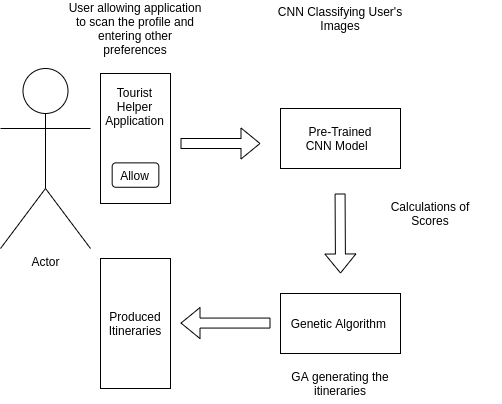
\includegraphics[scale=0.45]{Diagram.png}
    \label{diagram}
\end{figure}

  \section{The Dataset}
    A dataset of 2747 images was scraped from public Instagram posts from
hashtags by using Puppeteer \footnote{\url{https://pptr.dev/}} (A javascript web-scraper). The dataset
consists of 5 classes, beach, clubbing, nature, drinks, football with
the potential to add more classes in the future. If a person’s image
post falls under a certain category, more activities leaning towards
that activity will be suggested in the itinerary and therefore a
person’s preferences are collected automatically from Instagram posts
and stories. The Beach dataset contains images of seaside, swimming
and summer related activities, the Nature dataset contains images
related to greenery and landscapes, the clubbing dataset contains
crowds and people dancing in a club, the drinks dataset contains
images of cocktails and people in a bar and the football dataset
contains images of stadiums for sport fans. 

    \begin{figure}[H]
        \caption{The image shows a sample image form each of the category}
        \centering
        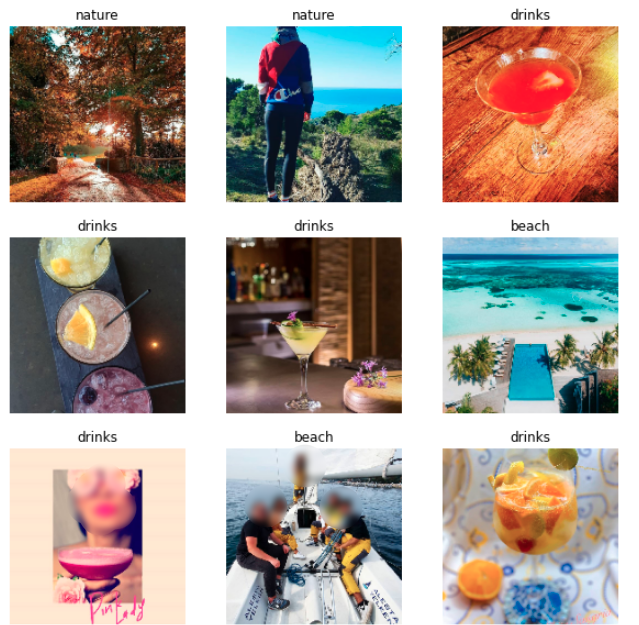
\includegraphics[scale=0.3]{dataset.png}
        \label{dataset}
    \end{figure}


  \section{Results and Evaluation Plan}
  \label{Evaluation}

  \bibliographystyle{IEEEtran}
  \bibliography{fypReferences}

\end{document}